% ── AI Chat ───────────────────────────────────────────────────
\chapter{AI Chat}

        AI~chat je najinováčnejšou súčasťou systému. Umožňuje používateľom klásť
otázky v~prirodzenom jazyku nad obsahom nahraných dokumentov.
Systém odpovie na základe extrahovaného textu z~vybraných súborov, čím výrazne
urýchľuje orientáciu v~rozsiahlych podkladoch.

\section{Integrácia AI}

        AI~chat sme v~aplikácii implementovali ako samostatnú komunikačnú vrstvu,
ktorá pracuje nad vybraným kontextom z~dokumentov, projektov a~úloh. Backend sme
postavili na lokálnom modeli cez službu Ollama~\cite{ollama_github}, pričom predvolený model je
\texttt{gemma4:26b}~\cite{gemma4_google}.

        Z~pohľadu ochrany údajov sme riešenie navrhli tak, aby zostalo čo najviac
vnútri infraštruktúry systému. Otázky používateľa sa spracúvajú lokálne a~model
pracuje s~kontextom, ktorý je dostupný v~databáze aplikácie. Pri odpovediach sa
zohľadňuje aj história konkrétnej konverzácie, takže chat vie nadväzovať na
predchádzajúce otázky bez nutnosti opakovať celý kontext.

\section{Rozhranie chatu}

        Používateľské rozhranie AI~chatu sme rozdelili na dva hlavné panely. V~ľavej
časti sa nachádza história konverzácií, kde si používateľ môže prepnúť medzi
jednotlivými vláknami alebo založiť novú konverzáciu. Pravá časť obsahuje samotné
správy, vstupné pole a~ovládanie kontextu.

        Nový chat je možné vytvoriť buď prázdny, alebo s~pripojeným dokumentom.
Po otvorení konverzácie sa správy zobrazujú v~chronologickom poradí, pričom
odpovede asistenta sú formátované pomocou Markdownu. Tým sa výsledný text stáva
prehľadnejším a~ľahšie čitateľným najmä pri odrážkach, odkazoch alebo kratších
zhrnutiach (obr.~\ref{fig:ai_chat}).

\begin{figure}[H]
  \centering
  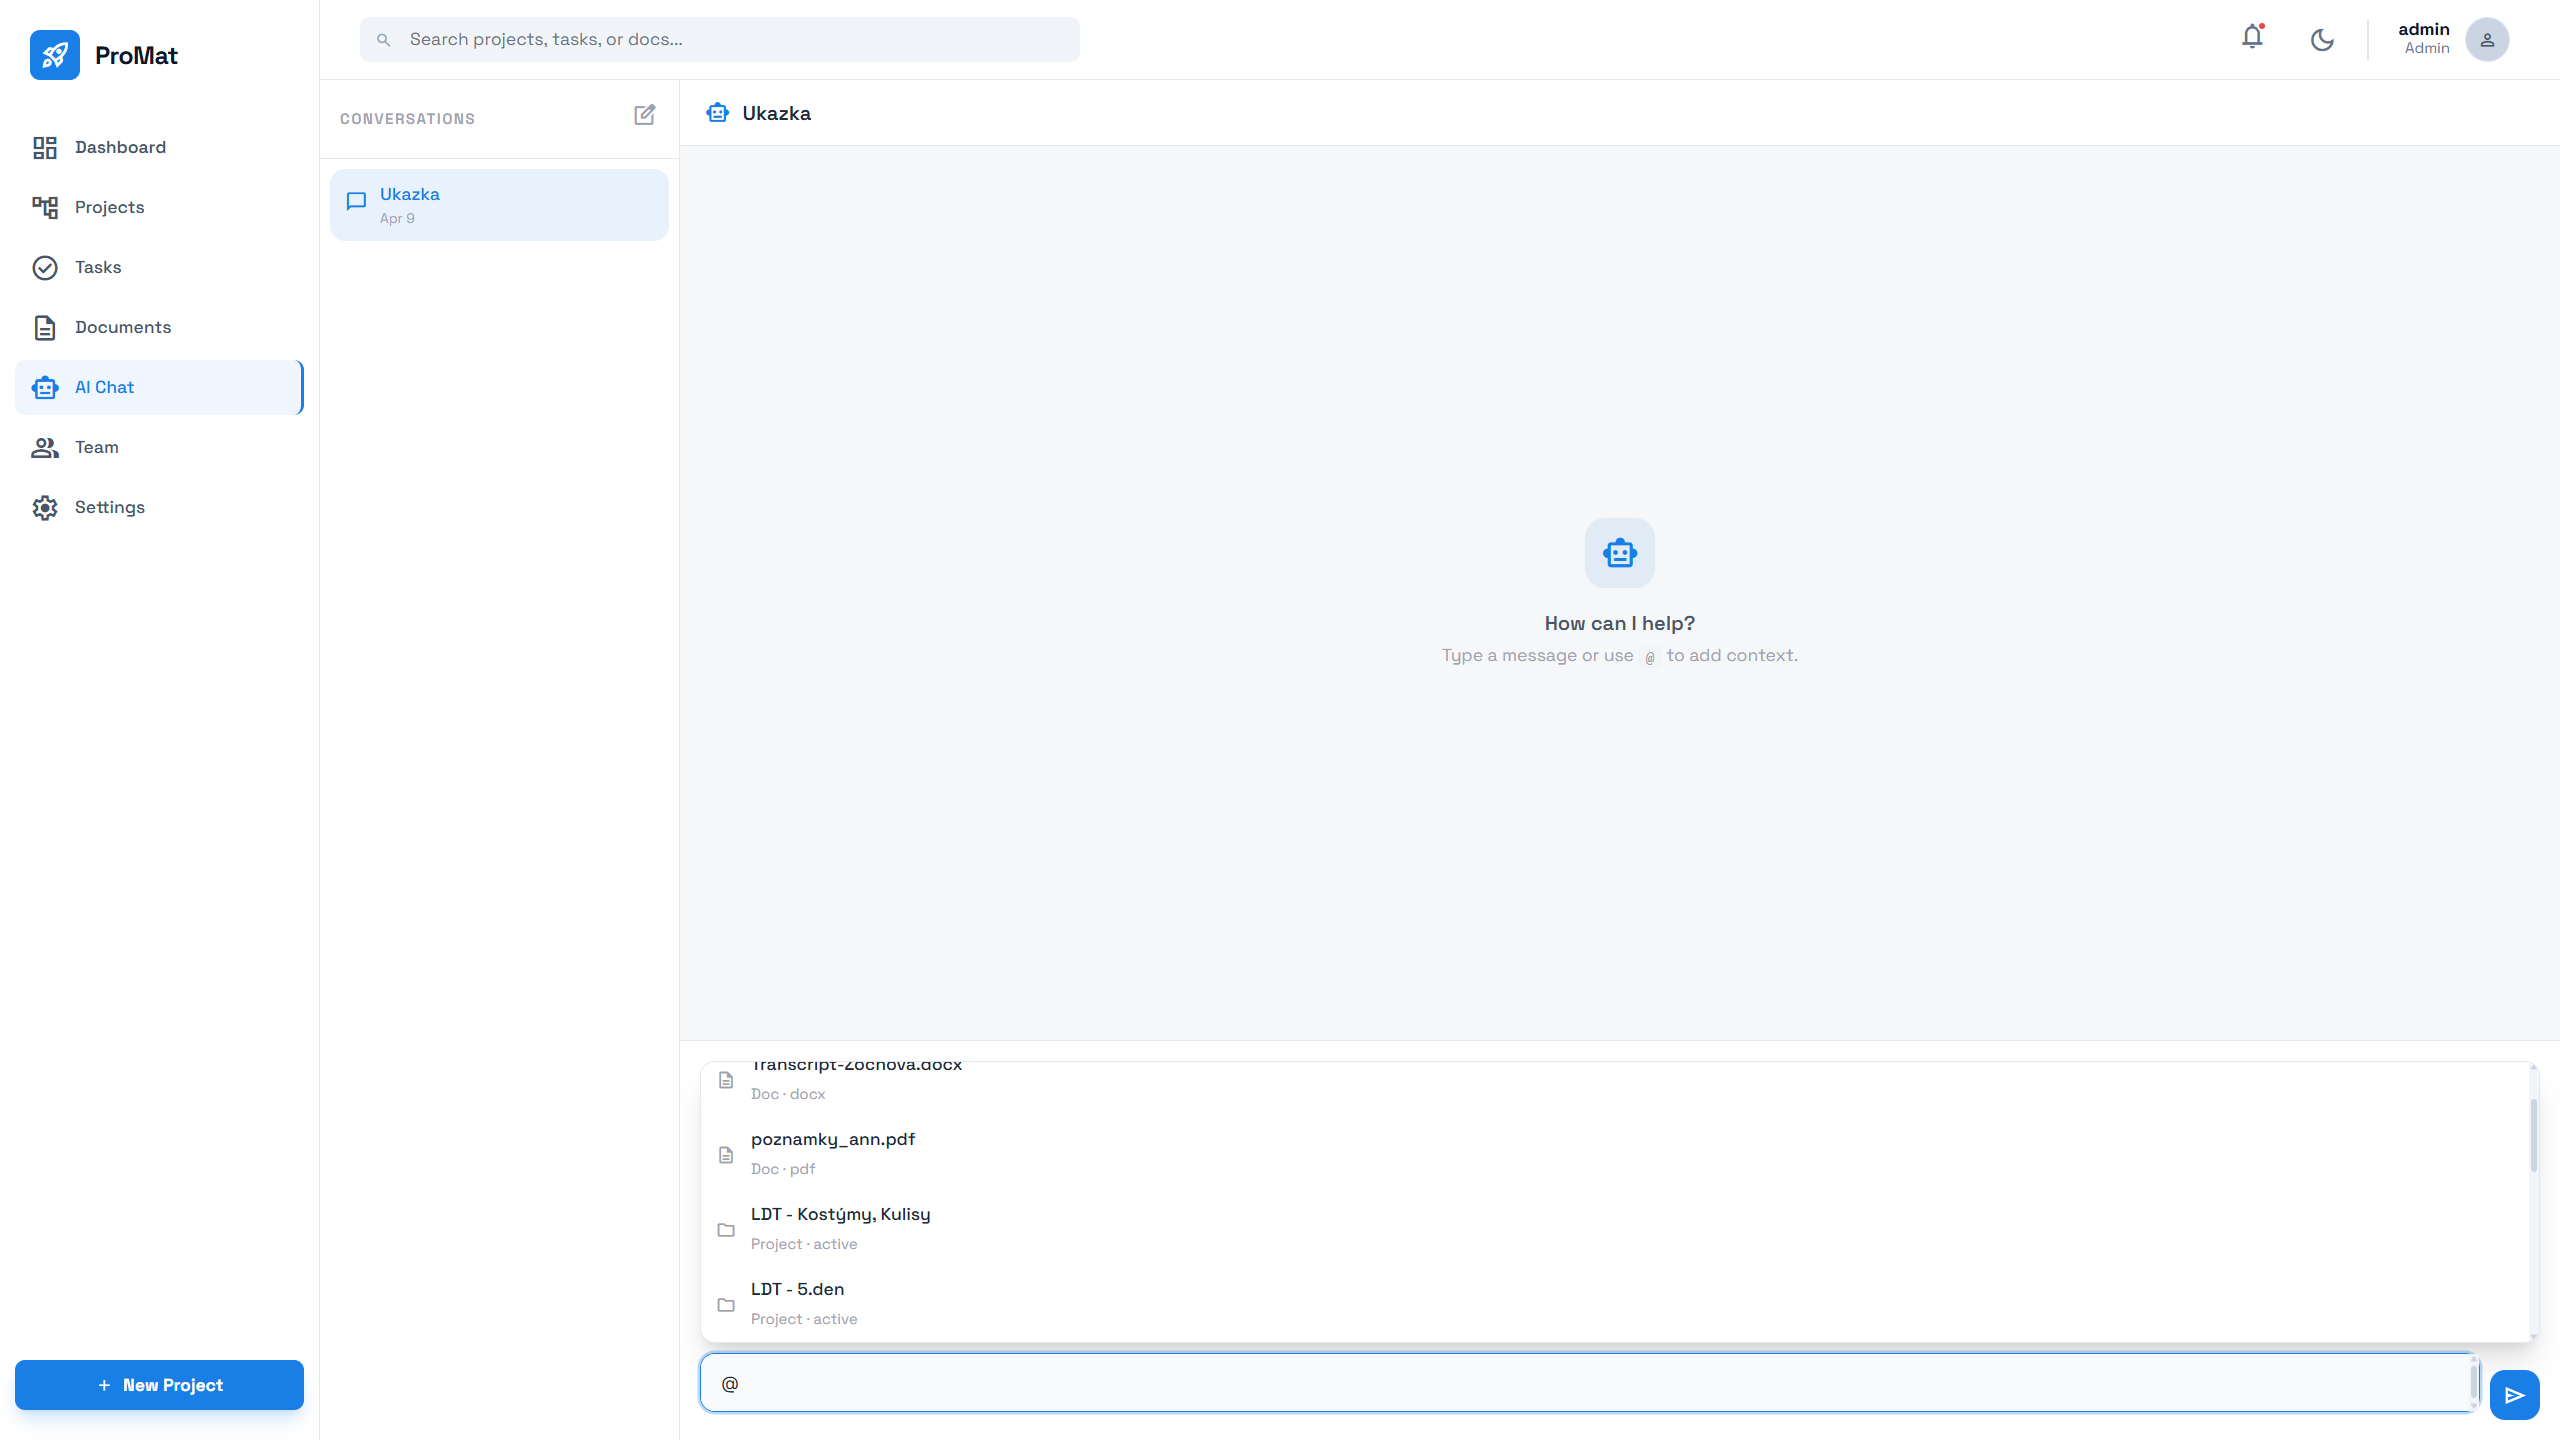
\includegraphics[width=0.9\textwidth]{images/ai_chat.png}
  \caption{Rozhranie AI~chatu}
  \label{fig:ai_chat}
\end{figure}

        Vstupné pole podporuje zadávanie zmienok pomocou znaku \texttt{@}. Po jeho
zadaní sa zobrazí načítavač dokumentov, projektov a~úloh, ktoré má používateľ
k~dispozícii. Po výbere položky sa vytvorí vizuálna značka a~do správy sa doplní
štruktúrovaná referencia, ktorú backend vie pri spracovaní preložiť na konkrétny
záznam v~databáze.

        Samotné odoslanie správy prebieha cez asynchrónne volanie bez obnovovania
stránky. Používateľ okamžite vidí svoju správu aj indikátor písania, následne sa
pridá odpoveď modelu. Pri nedostupnosti AI~backendu sa zobrazí chybové hlásenie,
aby bolo správanie systému zrozumiteľné aj pri výpadku služby (obr.~\ref{fig:ai_odpoved}).

\begin{figure}[H]
  \centering
  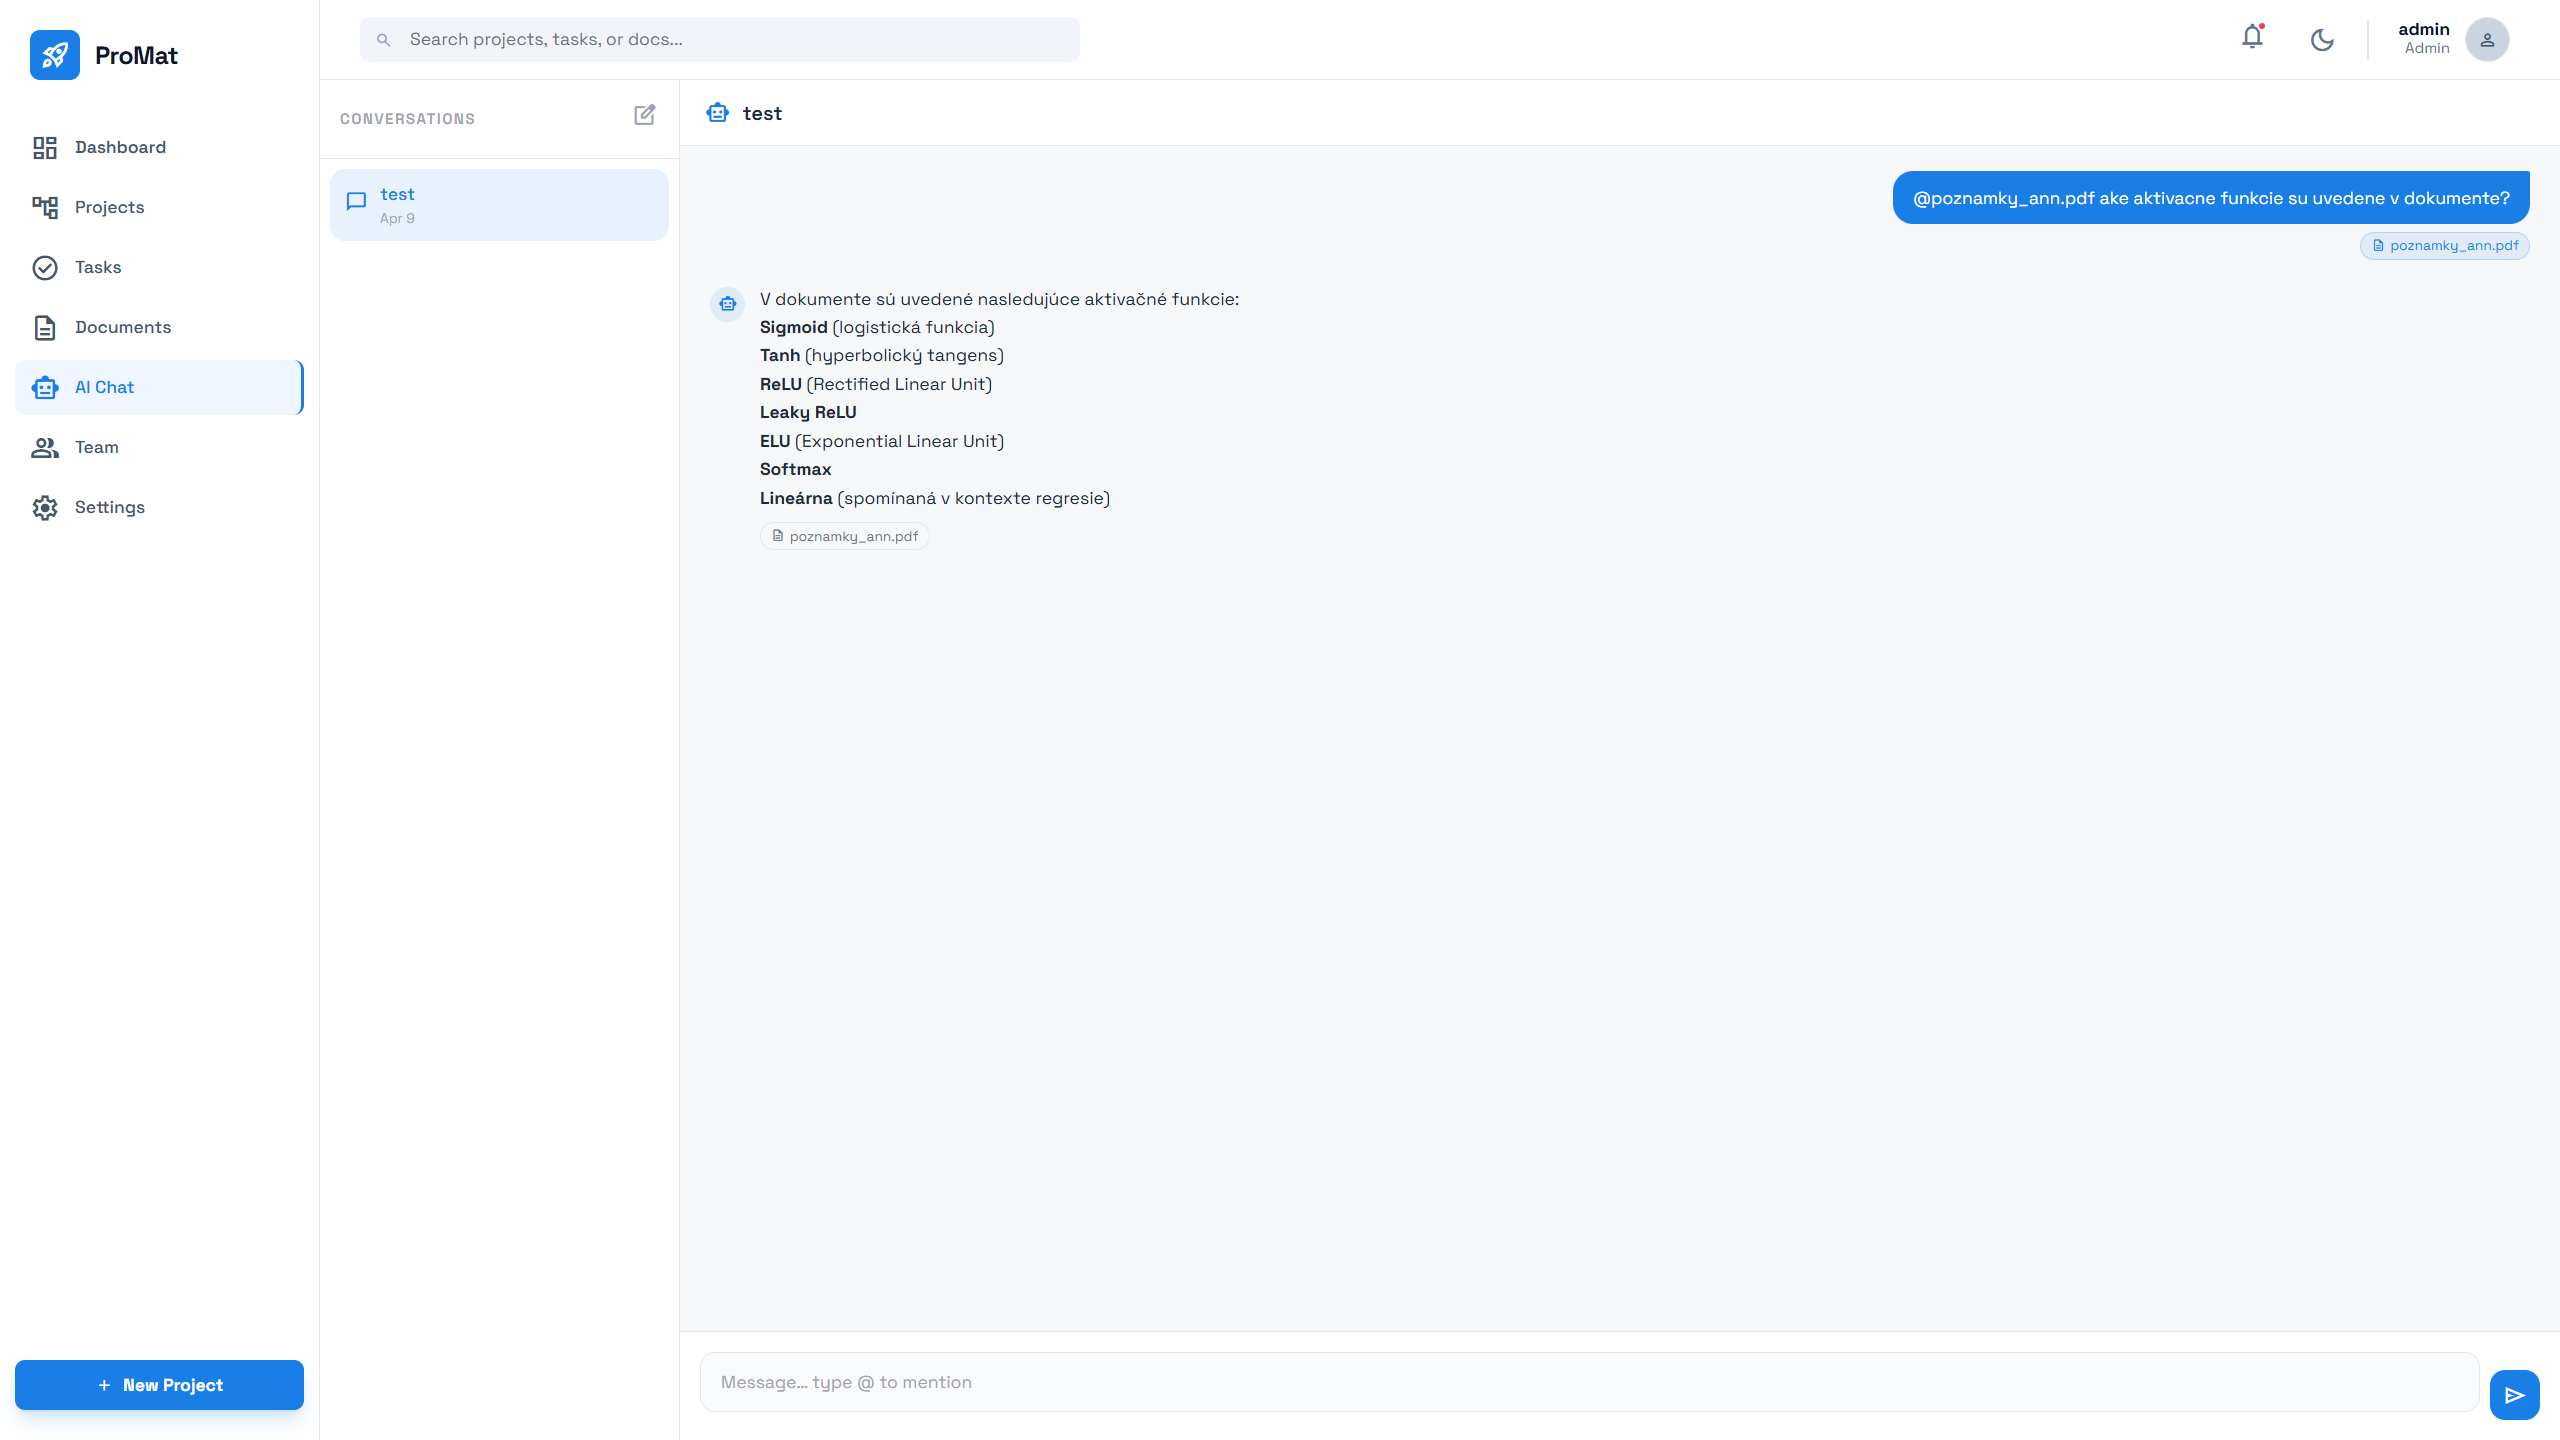
\includegraphics[width=0.9\textwidth]{images/ai_chat_odpoved.png}
  \caption{Príklad AI~odpovede nad obsahom dokumentu}
  \label{fig:ai_odpoved}
\end{figure}

        Na obrázku je vidieť, že odpoveď asistenta vie vychádzať z~pripojeného
dokumentu a~zároveň zachovávať kontext predchádzajúcej komunikácie. Tým sa AI~chat
stáva praktickým nástrojom na rýchle prehľadávanie obsahu bez nutnosti manuálneho
čítania celého súboru.
